\chapter{Neural Networks}
\label{chap:neural-networks}

\section{Network Architecture}
\label{sec:network-architecture}
	
	This section defines affine maps and shows why composing them alone never gives more expressive power than a single affine map, introduces componentwise activation functions and the resulting feedforward network architecture, and closes with the softmax output layer that turns a network's raw output into a categorical distribution. \\
	
	This is where the pieces built across the previous three chapters assemble into a single object: a network whose expressive power comes specifically from nonlinearity, not depth alone (Remark~\ref{rem:why-nonlinearity}), and whose output is provably a categorical distribution rather than merely something shaped like one (Proposition~\ref{prop:softmax-simplex}), which is what licenses training it by minimising cross-entropy as derived in Chapter~\ref{chap:probability} and previewed in Remark~\ref{rem:network-loss-preview}. \\
	
	The forward pass, which is the system that evaluates the network layer by layer from input to output (Remark~\ref{rem:forward-pass}), is implemented from scratch in C++ as \texttt{network.hpp} (Appendix~\ref{app:forward-pass}).
	
	\subsection{Affine Maps}
		
		\begin{definition}[Affine Map]
			\label{def:affine-map}
			Let $T:\mathbb{R}^n\to\mathbb{R}^m$ be a linear operator (Definition~\ref{def:linear-operator}), represented in the standard bases by a matrix $A\in\mathrm{Mat}(m,n,\mathbb{R})$ (Proposition~\ref{prop:matrix-representation}), and let $b\in\mathbb{R}^m$ be a fixed vector. The map $F:\mathbb{R}^n\to\mathbb{R}^m$ defined by
			\[
				F(x) := Ax + b
			\]
			is called an affine map. $A$ is the linear part of $F$ and $b$ is its translation (or bias).
		\end{definition}
		
		\begin{remark}
			\label{rem:affine-not-linear}
			An affine map $F(x)=Ax+b$ (Definition~\ref{def:affine-map}) is a linear operator (Definition~\ref{def:linear-operator}) only when $b=0$: for $b\neq0$, $F(0)=b\neq0$, violating linearity, which forces $T(0)=0$ (take $\mu=\nu=0$ in Definition~\ref{def:linear-operator}).
		\end{remark}
		
		\begin{proposition}[Composition of Affine Maps is Affine]
			\label{prop:affine-composition}
			Let $F_1:\mathbb{R}^n\to\mathbb{R}^m$ and $F_2:\mathbb{R}^m\to\mathbb{R}^k$ be affine maps (Definition~\ref{def:affine-map}), with $F_1(x)=A_1x+b_1$ and $F_2(y)=A_2y+b_2$. Then $F_2\circ F_1:\mathbb{R}^n\to\mathbb{R}^k$ is affine, with
			\[
				(F_2\circ F_1)(x) = (A_2A_1)x + (A_2b_1+b_2)
			\]
		\end{proposition}
		
		\begin{proof}
			By direct computation:
			\begin{align*}
				(F_2\circ F_1)(x) &= F_2(F_1(x)) \\
				&= F_2(A_1x+b_1) \\
				&= A_2(A_1x+b_1)+b_2 \\
				&= A_2A_1x + A_2b_1 + b_2 \\
				&= (A_2A_1)x + (A_2b_1+b_2)
			\end{align*}
			Here $A_2A_1$ is ordinary matrix multiplication, which by Corollary~\ref{cor:composition-multiplication} represents the composition of the linear operators $A_1,A_2$ correctly in the standard bases. 
			Setting $A:=A_2A_1$ and $b:=A_2b_1+b_2$ is exactly the form $F(x)=Ax+b$ of Definition~\ref{def:affine-map}, so $F_2\circ F_1$ is also affine with linear part $A_2A_1$ and translation $A_2b_1+b_2$.
		\end{proof}
		
		\begin{corollary}[Depth Collapse of Affine Compositions]
			\label{cor:affine-depth-collapse}
			Let $F_1,\dots,F_L$ be affine maps, with $F_\ell:\mathbb{R}^{n_{\ell-1}}\to\mathbb{R}^{n_\ell}$, $F_\ell(x)=A_\ell x+b_\ell$, for $\ell=1,\dots,L$. Then the composition
			\[
				F := F_L\circ\cdots\circ F_1 : \mathbb{R}^{n_0}\to\mathbb{R}^{n_L}
			\]
			is affine: there exist $A\in\mathrm{Mat}(n_L,n_0,\mathbb{R})$ and $b\in\mathbb{R}^{n_L}$ such that $F(x)=Ax+b$ for all $x$.
		\end{corollary}
		
		\begin{proof}
			We proceed by induction on $L$.
			
			Base Case:
			$F=F_1$ is affine by hypothesis.
			
			Inductive Step:
			Suppose $G:=F_{L-1}\circ\cdots\circ F_1$ is affine, say $G(x)=A'x+b'$ for some $A',b'$. Then
			\[
				F = F_L\circ G
			\]
			a composition of the two affine maps $G$ and $F_L$. By Proposition~\ref{prop:affine-composition}, $F_L\circ G$ is affine, with linear part $A_LA'$ and translation $A_Lb'+b_L$. So $F$ is affine, with $A:=A_LA'$, $b:=A_Lb'+b_L$.
			
			By induction, $F=F_L\circ\cdots\circ F_1$ is affine for every $L\ge1$.
		\end{proof}
		
		\begin{compremark}
			\texttt{network.hpp} implements \texttt{Network::forward()} in Appendix~\ref{app:forward-pass} as a loop over layers, applying each layer's affine map and activation in sequence. \\
			
			This is worth justifying against Corollary~\ref{cor:affine-depth-collapse}: layer 0 uses \texttt{identityScalar} and the output layer applies no activation (Definition~\ref{def:feedforward-network}), so no non-affine function appears anywhere, and by that corollary this two-layer network is guaranteed to collapse to a single affine map. \texttt{forward()} could skip the loop entirely here. It doesn't, because the collapse only holds when every activation is the identity: a nonlinearity like ReLU breaks it (Remark~\ref{rem:why-nonlinearity}), so the layer-by-layer structure is what has to generalise. This identity-activation case just gives a hand-computable answer to check that structure against, not a reason to shortcut it. \\
			
			Verified in \texttt{main()}: \texttt{net.forward(x0)} and the independently-computed $A_2(A_1x_0+b_1)+b_2$ both give $(32,-23)$, an exact match.
		\end{compremark}
		
	\subsection{Activation Functions}
		
		\begin{remark}[Nonlinearity is Necessary]
			\label{rem:why-nonlinearity}
			Corollary~\ref{cor:affine-depth-collapse} has a direct consequence for network architecture: if every layer of an $L$-layer network were purely affine, with no nonlinearity applied between layers, the entire network would collapse to a single affine map $F(x)=Ax+b$, which would be exactly as expressive as one layer. \\
			
			Depth alone, without nonlinearity interleaved between the affine maps, buys nothing no matter how many layers are stacked, the composition is indistinguishable from a single affine transformation of the input. This is why every layer of a network is followed by a nonlinear activation function, which is the subject of this next subsection.
		\end{remark}
		
		\begin{definition}[Activation Function]
			\label{def:activation}
			Let $\sigma:\mathbb{R}\to\mathbb{R}$ be a function. The activation of $\sigma$ on $\mathbb{R}^n$ is the map $\sigma:\mathbb{R}^n\to\mathbb{R}^n$ defined componentwise, i.e.\
			\[
				\sigma(x) := \big(\sigma(x_1),\dots,\sigma(x_n)\big) \qquad \text{for } x=(x_1,\dots,x_n)\in\mathbb{R}^n
			\]
			applying $\sigma$ independently to each coordinate of $x$, with no interaction between coordinates.
		\end{definition}
		
		\begin{example}[ReLU and Sigmoid]
			\label{ex:relu-sigmoid}
			Two activation functions (Definition~\ref{def:activation}) used throughout this chapter are:
			\begin{enumerate}[label=\roman*.]
				\item \label{ex:relu} The \emph{Rectified Linear Unit} (ReLU) \citep{NairHinton2010}:
				\[
					\mathrm{ReLU}(t) := \max(t,0) = \begin{cases} t & t\ge0 \\ 0 & t<0 \end{cases}
				\]
				\item \label{ex:sigmoid} The \emph{Sigmoid} function:
				\[
					\varsigma(t)  := \frac{1}{1+e^{-t}}
				\]
			\end{enumerate}
			Both are applied componentwise on $\mathbb{R}^n$ per Definition~\ref{def:activation}: for $x=(x_1,\dots,x_n)\in\mathbb{R}^n$, $\mathrm{ReLU}(x) = (\mathrm{ReLU}(x_1),\dots,\mathrm{ReLU}(x_n))$, and likewise for $\varsigma$.
		\end{example}
		
		\begin{remark}[Non-Differentiability of ReLU at $0$]
			\label{rem:relu-nondifferentiable}
			$\mathrm{ReLU}(t)=\max(t,0)$ (Example~\ref{ex:relu-sigmoid}, \ref{ex:relu}) is not differentiable at $t=0$: the one-sided derivatives are $0$ (approaching from below) and $1$ (approaching from above), which disagree. So the Chain Rule (Theorem~\ref{thm:chain-rule}) does not literally apply at any point where an intermediate quantity equals exactly $0$ after a ReLU is applied. \\
			
			In practice, this is resolved by adopting the convention:
			\[
				\mathrm{ReLU}'(0) := 0
			\]
			and treating $\mathrm{ReLU}$ as differentiable everywhere else, with $\mathrm{ReLU}'(t)=1$ for $t>0$ and $\mathrm{ReLU}'(t)=0$ for $t<0$. This is a convention, not a mathematical fact derived from Theorem~\ref{thm:chain-rule} or any other result in this paper: the single point $t=0$ has measure zero and is reached only for specific inputs, so the convention has no practical effect on computation, but it is not rigorously justified by the calculus developed in Chapter~\ref{chap:calculus}.
		\end{remark}
		
	\subsection{Feedforward Networks}
		
		\begin{definition}[Feedforward Network]
			\label{def:feedforward-network}
			Let $L\ge1$ be an integer (the depth), and let $n_0,n_1,\dots,n_L$ be positive integers (the widths of each layer). For each $\ell=1,\dots,L$, let $A_\ell\in\mathrm{Mat}(n_\ell,n_{\ell-1},\mathbb{R})$ and $b_\ell\in\mathbb{R}^{n_\ell}$, defining the affine map $F_\ell(x):=A_\ell x+b_\ell$ (Definition~\ref{def:affine-map}), and let $\sigma:\mathbb{R}\to\mathbb{R}$ be an activation function (Definition~\ref{def:activation}). Write
			\[
				\theta := (A_1,b_1,\dots,A_L,b_L)
			\]
			for the collection of all these matrices and vectors, the parameters of the network.
			
			Given an input $x_0\in\mathbb{R}^{n_0}$ (the data, not a parameter), define, for $\ell=1,\dots,L$,
			\[
				z_\ell := F_\ell(x_{\ell-1}) = A_\ell x_{\ell-1}+b_\ell \qquad \text{(the \emph{pre-activation} at layer $\ell$)}
			\]
			\[
				x_\ell := \begin{cases} \sigma(z_\ell) & \ell < L \\ z_\ell & \ell = L \end{cases} \qquad \text{(the \emph{post-activation} at layer $\ell$)}
			\]
			applying $\sigma$ componentwise (Definition~\ref{def:activation}). The resulting map
			\[
				f_\theta : \mathbb{R}^{n_0}\to\mathbb{R}^{n_L} \qquad f_\theta(x_0) := x_L
			\]
			is the feedforward network with parameters $\theta$.
		\end{definition}
		
		\begin{figure}[htbp]
			\centering
			\begin{tikzpicture}[node distance=1.2cm, >=stealth]
				% Input layer: 784 nodes, reduced to 5 + vdots
				\foreach \i in {1,2,3,4}
				\node[circle, draw, minimum size=0.5cm] (L0-\i) at (0, -\i*0.7) {};
				\node (L0-dots) at (0, -4*0.7-0.5) {$\vdots$};
				\node[circle, draw, minimum size=0.5cm] (L0-6) at (0, -4*0.7-1.3) {};
				
				% Hidden layer: 128 nodes, reduced to 5 + vdots
				\foreach \i in {1,2,3,4}
				\node[circle, draw, minimum size=0.5cm] (L1-\i) at (3, -\i*0.7-0.3) {};
				\node (L1-dots) at (3, -4*0.7-0.8) {$\vdots$};
				\node[circle, draw, minimum size=0.5cm] (L1-6) at (3, -4*0.7-1.6) {};
				
				% Output layer: all 10 nodes
				\foreach \i in {1,...,10}
				\node[circle, draw, minimum size=0.5cm] (L2-\i) at (6, -\i*0.55) {};
				
				% Edges: input -> hidden (only drawn to/from the visible nodes, not \vdots)
				\foreach \i in {1,2,3,4,6}
				\foreach \j in {1,2,3,4,6}
				\draw[->] (L0-\i) -- (L1-\j);
				
				% Edges: hidden -> output
				\foreach \i in {1,2,3,4,6}
				\foreach \j in {1,...,10}
				\draw[->] (L1-\i) -- (L2-\j);
				
				% Labels
				\node[below=0.3cm of L0-6] {$x_0 \in \mathbb{R}^{784}$};
				\node[below=0.3cm of L1-6] {$x_1 \in \mathbb{R}^{128}$};
				\node[below=0.3cm of L2-10] {$x_2 \in \mathbb{R}^{10}$};
				
				\node[above] at (1.5, 0.2) {$A_1, b_1$};
				\node[above] at (4.5, 0.2) {$A_2, b_2$};
			\end{tikzpicture}
			\caption{The feedforward network (Definition~\ref{def:feedforward-network}) used later in this paper: an input layer of $784$ nodes ($x_0\in\mathbb{R}^{784}$), a hidden layer of $128$ nodes ($x_1\in\mathbb{R}^{128}$) with ReLU activation, and an output layer of $10$ nodes ($x_2\in\mathbb{R}^{10}$). Each arrow bundle represents the affine map $A_\ell x_{\ell-1}+b_\ell$; the nonlinearity is applied at the nodes it feeds into, not on the arrows themselves.}
			\label{fig:network-diagram}
		\end{figure}
		
		\begin{remark}[The Forward Pass]
			\label{rem:forward-pass}
			Evaluating $f_\theta(x_0)$ (Definition~\ref{def:feedforward-network}), computing $x_1,x_2,\dots,x_L$ in order from a given input $x_0$, is called the forward pass. Writing it out,
			\[
				f_\theta = F_L \circ \sigma \circ F_{L-1} \circ \sigma \circ \cdots \circ \sigma \circ F_1
			\]
			makes explicit what Definition~\ref{def:feedforward-network} already encodes: a feedforward network is precisely an alternating composition of affine maps (Definition~\ref{def:affine-map}) and activations (Definition~\ref{def:activation}), exactly the kind of object this section set out to build.
		\end{remark}
		
		\begin{remark}[Parameter Count]
			\label{rem:parameter-count}
			The total number of scalar parameters in $\theta=(A_1,b_1,\dots,A_L,b_L)$ (Definition~\ref{def:feedforward-network}) is
			\[
				\sum_{\ell=1}^{L} \big(n_\ell n_{\ell-1} + n_\ell\big)
			\]
			since $A_\ell\in\mathrm{Mat}(n_\ell,n_{\ell-1},\mathbb{R})$ contributes $n_\ell n_{\ell-1}$ entries and $b_\ell\in\mathbb{R}^{n_\ell}$ contributes $n_\ell$ entries, at each layer $\ell$.
		\end{remark}
		
	\subsection{The Softmax Output Layer}
		
		\begin{definition}[Softmax]
			\label{def:softmax}
			The softmax function is the map $\mathrm{softmax}:\mathbb{R}^K\to\mathbb{R}^K$ defined by
			\[
				\mathrm{softmax}(z)_k := \frac{e^{z_k}}{\sum_{j=1}^K e^{z_j}} \qquad \text{for } k=1,\dots,K
			\]
			for $z=(z_1,\dots,z_K)\in\mathbb{R}^K$.
		\end{definition}
		
		\begin{proposition}[Softmax Output as a Valid Categorical Parameter]
			\label{prop:softmax-simplex}
			For any $z\in\mathbb{R}^K$, the vector $p:=\mathrm{softmax}(z)$ (Definition~\ref{def:softmax}) satisfies $p_k\ge0$ for every $k$ and $\sum_{k=1}^Kp_k=1$, which are the conditions Definition~\ref{def:categorical-distribution} requires of a parameter $p$.
		\end{proposition}
		
		\begin{proof}
			By Definition~\ref{def:softmax}, $p_k = e^{z_k}/\sum_{j=1}^Ke^{z_j}$ for each $k$. Since $e^{z_k}>0$ for every real $z_k$, and the denominator $\sum_je^{z_j}$ is a sum of such positive terms, $p_k>0$ (in particular $p_k\ge0$) for every $k$.
			
			Summing,
			\[
				\sum_{k=1}^K p_k = \sum_{k=1}^K \frac{e^{z_k}}{\sum_{j=1}^Ke^{z_j}} = \frac{\sum_{k=1}^Ke^{z_k}}{\sum_{j=1}^Ke^{z_j}} = 1
			\]
			since the numerator and denominator are the same sum.
			
			So $p=\mathrm{softmax}(z)$ satisfies both conditions of Definition~\ref{def:categorical-distribution}.
		\end{proof}
		
		\begin{proposition}[Shift Invariance of Softmax]
			\label{prop:softmax-shift-invariance}
			For any $z\in\mathbb{R}^K$ and $c\in\mathbb{R}$,
			\[
				\mathrm{softmax}(z+c\mathbbm{1}) = \mathrm{softmax}(z)
			\]
			where $z+c\mathbbm{1} := (z_1+c,\dots,z_K+c)$.
		\end{proposition}
		
		\begin{proof}
			By Definition~\ref{def:softmax}, for each $k$,
			\[
				\mathrm{softmax}(z+c\mathbbm{1})_k = \frac{e^{z_k+c}}{\sum_{j=1}^Ke^{z_j+c}} = \frac{e^{z_k}e^c}{\sum_{j=1}^Ke^{z_j}e^c} = \frac{e^c\, e^{z_k}}{e^c\sum_{j=1}^Ke^{z_j}} = \frac{e^{z_k}}{\sum_{j=1}^Ke^{z_j}} = \mathrm{softmax}(z)_k
			\]
			using $e^{z_j+c}=e^{z_j}e^c$ and cancelling the common factor $e^c$ from numerator and denominator.
		\end{proof}
		
		\begin{compremark}
			\texttt{network.hpp} (Appendix~\ref{app:forward-pass}) also implements \texttt{softmax()}, which subtracts $m$, the maximum logit, before calling \texttt{std::exp}. \\
			
			This is justified by Proposition~\ref{prop:softmax-shift-invariance}: subtracting any constant $c$ leaves softmax's output unchanged, so subtracting $m$ is not an approximation as it's one exact member of a family the proposition already guarantees is correct. It's the safest member, though: subtracting $m$ keeps the largest exponent at $e^0=1$, so nothing overflows, unlike subtracting nothing when logits are large. \\
			
			Verified in \texttt{main()}: with logits as far apart as $32$ and $-23$, \texttt{softmax}'s output still summed to exactly $1$ (Proposition~\ref{prop:softmax-simplex}), with one entry rounding to $\approx1.3\times10^{-24}$.
		\end{compremark}
		
		\begin{remark}[The Loss Function is Cross-Entropy]
			\label{rem:network-loss-preview}
			Applying softmax to the network's output, $Q_\theta(x):=\mathrm{softmax}(f_\theta(x))$, produces a valid categorical parameter for every input $x$ (Proposition~\ref{prop:softmax-simplex}), exactly the object anticipated in Remark~\ref{rem:categorical-mle-to-network}.
			
			For a training pair $(x^{(i)},y^{(i)})$, with $\hat p^{(i)}$ the one-hot distribution on the observed label $y^{(i)}$, the same argument behind Corollary~\ref{cor:mle-min-cross-entropy} gives a per-example loss $H(\hat p^{(i)},Q_\theta(x^{(i)}))$; summing over the training set gives the objective
			\[
				\sum_i H\big(\hat p^{(i)}, Q_\theta(x^{(i)})\big)
			\]
			So the loss used to train this network in Section~\ref{sec:loss-function} is cross-entropy by derivation, not convention: applying the Chapter~\ref{chap:probability} argument example-by-example rather than to one shared distribution.
			
			This per-example extension of Corollary~\ref{cor:mle-min-cross-entropy} is not itself proved anywhere in this document; it is stated here as a direct analogue of the cited result, not a cited consequence of it.
		\end{remark}
	
\section{Backpropagation}
\label{sec:backpropagation}
	
	This section formalises the network's training objective as cross-entropy loss (Section~\ref{sec:loss-function}), then derives the backward pass: the recursion for the per-layer error term $\delta_\ell$ and the resulting gradients of the loss with respect to every layer's weights and biases via the chain rule established in Chapter~\ref{chap:calculus} (Section~\ref{sec:backward-pass}). \\
	
	This is where the paper's central claim is settled: backpropagation is not a separate algorithm bolted onto the network, it is Theorem~\ref{thm:chain-rule} applied repeatedly \citep{RumelhartHintonWilliams1986}, layer by layer and every gradient a training run computes is provably the true gradient of the loss this chapter derived from maximum likelihood, not an approximation or a heuristic. \\
	
	The corresponding C++ implementation, shared between the forward and backward pass, is in \texttt{network.hpp} (Appendix~\ref{app:forward-pass}), with the backward pass specifically verified in \texttt{backward\allowbreak\_pass.cpp} (Appendix~\ref{app:backward-pass}).
	
	\subsection{The Loss Function}
	\label{sec:loss-function}
	
		\begin{definition}[Training Loss]
			\label{def:training-loss}
			Let $\{(x^{(i)},y^{(i)})\}_{i=1}^n$ be a training set, with each $y^{(i)}$ a class label in $\{1,\dots,K\}$, where $K=n_L$ is the network's output width (Definition~\ref{def:feedforward-network}). Write $\hat p^{(i)}$ for the one-hot distribution on the observed label $y^{(i)}$, i.e.\ $\hat p^{(i)}_k=1$ if $k=y^{(i)}$ and $\hat p^{(i)}_k=0$ otherwise, and $Q_\theta(x):=\mathrm{softmax}(f_\theta(x))$ (Remark~\ref{rem:network-loss-preview}). The training loss is
			\[
				L(\theta) := \sum_{i=1}^n H\big(\hat p^{(i)}, Q_\theta(x^{(i)})\big)
			\]
			the sum of per-example cross-entropy terms \citep{GoodfellowBengioCourville2016}.
		\end{definition}
		
		\begin{remark}[Training Loss in Closed Form]
			\label{rem:training-loss-closed-form}
			Since $\hat p^{(i)}$ is one-hot on $y^{(i)}$, every term in $H(\hat p^{(i)},Q_\theta(x^{(i)}))=-\sum_k\hat p^{(i)}_k\log Q_\theta(x^{(i)})_k$ vanishes except $k=y^{(i)}$ (Definition~\ref{def:training-loss}), so
			\[
				L(\theta) = -\sum_{i=1}^n \log Q_\theta(x^{(i)})_{y^{(i)}}
			\]
		\end{remark}
		
		\begin{remark}[Reduction to a Single Example]
			\label{rem:loss-single-example}
			By linearity of differentiation, computing $\nabla_\theta L(\theta)$ (Definition~\ref{def:training-loss}) reduces to computing the gradient of a single term, $-\log Q_\theta(x)_y$, and summing over the training set. The next section, Section~\ref{sec:backward-pass}, derives this gradient for one example, dropping the $(i)$ superscript accordingly.
		\end{remark}
		
	\subsection{The Backward Pass}
	\label{sec:backward-pass}
		
		\begin{definition}[Backward Error Term]
			\label{def:backward-error}
			Fix a single training example $(x,y)$, dropping the $(i)$ superscript as in the closing remark of the above section, Section~\ref{sec:loss-function}. For each layer $\ell=1,\dots,L$, the backward error term at layer $\ell$ is
			\[
				\delta_\ell := \frac{\partial L}{\partial z_\ell}
			\]
			the gradient of the loss with respect to that layer's pre-activation (Definition~\ref{def:feedforward-network}).
		\end{definition}
		
		\begin{proposition}[Output-Layer Error Term]
			\label{prop:output-layer-error}
			The output layer error term is
			\[
				\delta_L = Q_\theta(x) - \hat p
			\]
		\end{proposition}
		
		\begin{proof}
			$L = -\log Q_\theta(x)_y = -\log\mathrm{softmax}(z_L)_y = -z_{L,y} + \log\sum_{j=1}^K e^{z_{L,j}}$ (Definition~\ref{def:softmax}). Differentiating with respect to $(z_L)_k$, by cases:
			
			If $k=y$: $\dfrac{\partial L}{\partial(z_L)_k} = -1 + \dfrac{e^{z_{L,k}}}{\sum_je^{z_{L,j}}} = Q_\theta(x)_k - 1$.
			
			If $k\neq y$: $\dfrac{\partial L}{\partial(z_L)_k} = 0 + \dfrac{e^{z_{L,k}}}{\sum_je^{z_{L,j}}} = Q_\theta(x)_k$.
			
			In both cases, since $\hat p_k=1$ if $k=y$ and $0$ otherwise, this is $Q_\theta(x)_k - \hat p_k$. So $\delta_L = Q_\theta(x)-\hat p$.
		\end{proof}
		
		\begin{definition}[Hadamard Product]
			\label{def:hadamard-product}
			For $u,v\in\mathbb{R}^n$, the Hadamard product $u\odot v\in\mathbb{R}^n$ is defined entrywise by $(u\odot v)_j := u_jv_j$.
		\end{definition}
		
		\begin{theorem}[Backward Recursion]
			\label{thm:backward-recursion}
			For $\ell=1,\dots,L-1$,
			\[
				\delta_\ell = \big(A_{\ell+1}^\top\delta_{\ell+1}\big) \odot \sigma'(z_\ell)
			\]
		\end{theorem}
		
		\begin{proof}
			By the Chain Rule (Theorem~\ref{thm:chain-rule}) applied through $z_\ell \to x_\ell \to z_{\ell+1}$: since $x_\ell=\sigma(z_\ell)$ (componentwise, Definition~\ref{def:activation}) and $(z_{\ell+1})_j = \sum_m(A_{\ell+1})_{jm}(x_\ell)_m + (b_{\ell+1})_j$, for each coordinate $k$,
			\[
				(\delta_\ell)_k = \frac{\partial L}{\partial(z_\ell)_k} = \sum_j \frac{\partial L}{\partial(z_{\ell+1})_j} \frac{\partial(z_{\ell+1})_j}{\partial(x_\ell)_k} \frac{\partial(x_\ell)_k}{\partial(z_\ell)_k} = \sum_j (\delta_{\ell+1})_j(A_{\ell+1})_{jk} \sigma'((z_\ell)_k)
			\]
			using $\partial(z_{\ell+1})_j/\partial(x_\ell)_k=(A_{\ell+1})_{jk}$ and, since $(x_\ell)_k=\sigma((z_\ell)_k)$ depends only on coordinate $k$ (Definition~\ref{def:activation}), $\partial(x_\ell)_k/\partial(z_\ell)_k=\sigma'((z_\ell)_k)$. This is
			\[
				(\delta_\ell)_k = \big(A_{\ell+1}^\top\delta_{\ell+1}\big)_k \sigma'((z_\ell)_k)
			\]
			i.e.\ $\delta_\ell = (A_{\ell+1}^\top\delta_{\ell+1})\odot\sigma'(z_\ell)$ (Definition~\ref{def:hadamard-product}). When $\sigma=\mathrm{ReLU}$, $\sigma'((z_\ell)_k)$ at any coordinate where $(z_\ell)_k=0$ is understood via the convention $\mathrm{ReLU}'(0):=0$ (Remark~\ref{rem:relu-nondifferentiable}).
		\end{proof}
		
		\begin{compremark}
			\texttt{backwardStep()} in \texttt{network.hpp}, Appendix~\ref{app:backward-pass}, implements Theorem~\ref{thm:backward-recursion}.
			
			It reuses \texttt{applyActivation()}, the same componentwise-apply function used to compute $\sigma(z_\ell)$ during the forward pass, to compute $\sigma'(z_\ell)$ as well, simply by passing it a different function pointer. 
			
			This is justified directly by Definition~\ref{def:activation}: componentwise application doesn't care what scalar function it's given, $\sigma$ or $\sigma'$, only that it's applied coordinate-by-coordinate with no interaction between them, so the same generic machinery correctly computes either.
			
			This is verified by the gradient check at \texttt{net.layers[0].A(0,0)}: numerical $0.853139$ against analytic $0.853139$, a difference of $6.3396\times10^{-12}$. This is the one non-degenerate check among those run, the entry whose gradient depends on the recursion propagating $\delta$ backward through both layers, so it is the check that genuinely stresses Theorem~\ref{thm:backward-recursion} rather than confirming a simpler, more local computation.
		\end{compremark}
		
		\begin{proposition}[Parameter Gradients]
			\label{prop:parameter-gradients}
			For $\ell=1,\dots,L$,
			\[
				\frac{\partial L}{\partial A_\ell} = \delta_\ell x_{\ell-1}^\top, \qquad \frac{\partial L}{\partial b_\ell} = \delta_\ell
			\]
		\end{proposition}
		
		\begin{proof}
			Since $(z_\ell)_j = \sum_k(A_\ell)_{jk}(x_{\ell-1})_k + (b_\ell)_j$, for each entry $(A_\ell)_{jk}$,
			\[
				\frac{\partial L}{\partial(A_\ell)_{jk}} = \frac{\partial L}{\partial(z_\ell)_j} \frac{\partial(z_\ell)_j}{\partial(A_\ell)_{jk}} = (\delta_\ell)_j(x_{\ell-1})_k
			\]
			which is exactly the $(j,k)$ entry of $\delta_\ell x_{\ell-1}^\top$, so $\partial L/\partial A_\ell = \delta_\ell x_{\ell-1}^\top$. Similarly, $\partial(z_\ell)_j/\partial(b_\ell)_j=1$, so $\partial L/\partial(b_\ell)_j=(\delta_\ell)_j$, i.e.\ $\partial L/\partial b_\ell=\delta_\ell$.
		\end{proof}
		
		\begin{compremark}
			\texttt{parameterGradients()} in \texttt{network.hpp}, Appendix~\ref{app:backward-pass}, implements Proposition~\ref{prop:parameter-gradients}.
			
			The outer product $\delta_\ell x_{\ell-1}^\top$ is computed directly via the existing \texttt{Matrix} \texttt{operator*} and \texttt{.transpose()}, rather than a dedicated outer-product routine: since \texttt{operator*} already handles matrix multiplication for any compatible dimensions, a column vector times a row vector is already exactly what it computes, so no special-cased routine is needed.
			
			Verified by \texttt{net.layers[1].A(1,2)} and \texttt{net.layers[0].b(2,0)}, both exactly $0$: the third hidden unit's pre-activation is negative ($z_1(2)=-0.25$), so $\mathrm{ReLU}'$ is $0$ there (Remark~\ref{rem:relu-nondifferentiable}), zeroing the corresponding entry of $\delta_1$ via the backward recursion (Theorem~\ref{thm:backward-recursion}) and propagating through to both formulas exactly.
		\end{compremark}
		
		\begin{remark}[Backpropagation]
			\label{rem:backpropagation}
			Computing the network's output requires one forward sweep through the layers $\ell=1,\dots,L$, producing every $z_\ell,x_\ell$ (Remark~\ref{rem:forward-pass}). \\
			
			Afterward, $\delta_L$ is computed first (Proposition~\ref{prop:output-layer-error}), then Theorem~\ref{thm:backward-recursion} gives $\delta_{L-1},\dots,\delta_1$ in order, traversing the layers opposite to the forward sweep. This is the reason for the name: the error term propagates backward, against the direction the input flowed forward. \\
			
			The gradients are not a separate pass: at each layer $\ell$, Proposition~\ref{prop:parameter-gradients} gives $\partial L/\partial A_\ell$ and $\partial L/\partial b_\ell$ directly from $\delta_\ell$ and the cached $x_{\ell-1}$, so every gradient falls out of the same backward sweep: one forward pass plus one backward pass, total, regardless of $L$. \\
			
			This two-phase procedure, forward to compute the output, backward to read off the error terms and gradients together, is what the term backpropagation refers to.
		\end{remark}
	
\section{Universal Approximation}
\label{sec:universal-approximation}
	
	This section constructs a single-hidden-layer ReLU network that approximates any continuous function on a compact interval to arbitrary accuracy, by building tent functions from ReLUs, showing their sums interpolate a target function, bounding the interpolation error via uniform continuity, and assembling these into the Universal Approximation Theorem. \\
	
	This closes a gap the rest of this chapter leaves open. Sections~\ref{sec:backpropagation} and \ref{sec:network-architecture} built the network architecture and showed how to train it, but neither addresses whether the architecture can represent what training is asked to find in the first place. \\
	
	Chapter~\ref{chap:calculus}'s gradient descent convergence theorem answers whether training can find a good solution, given one exists; this section answers whether one exists at all. It also depends specifically on the choice made in Section~\ref{sec:network-architecture} (Example~\ref{ex:relu-sigmoid}): the entire construction rests on ReLU's piecewise-linear shape, which is exactly what makes tent functions expressible as a finite sum of ReLUs (Proposition~\ref{prop:tent-relu}) whereas a smooth activation like sigmoid would not admit nearly as direct a construction.

	\subsection{Tent Functions}
		
		\begin{definition}[Tent Function]
			\label{def:tent-function}
			Let $x_{k-1}<x_k<x_{k+1}$ be three points. The tent function $T_k:\mathbb{R}\to\mathbb{R}$ is the piecewise-linear function that is $0$ outside the interval $[x_{k-1},x_{k+1}]$, rises linearly from $0$ to $1$ on $[x_{k-1},x_k]$, and falls linearly from $1$ to $0$ on $[x_k,x_{k+1}]$.
		\end{definition}
		
		\begin{figure}[h]
			\centering
			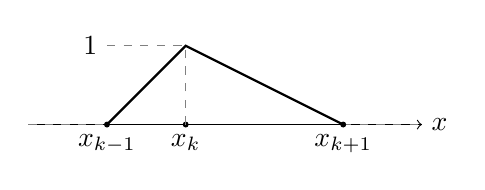
\begin{tikzpicture}
				
				% x-axis
				\draw[->] (-1,0) -- (4,0) node[right] {$x$};
				
				% Dashed zero-line reinforcing "zero outside [x_{k-1}, x_{k+1}]"
				\draw[dashed, gray] (-1,0) -- (0,0);
				\draw[dashed, gray] (3,0) -- (4,0);
				
				% The tent itself: two line segments
				\draw[thick] (0,0) -- (1,1) -- (3,0);
				
				% Points on the x-axis
				\filldraw (0,0) circle (0.03) node[below] {$x_{k-1}$};
				\filldraw (1,0) circle (0.03) node[below] {$x_k$};
				\filldraw (3,0) circle (0.03) node[below] {$x_{k+1}$};
				
				% Peak height label
				\draw[dashed, gray] (1,0) -- (1,1);
				\node[left] at (0,1) {$1$};
				\draw[dashed, gray] (0,1) -- (1,1);
				
			\end{tikzpicture}
			\caption{The tent function $T_k$ (Definition~\ref{def:tent-function}) for the asymmetric choice $x_{k-1}=0$, $x_k=1$, $x_{k+1}=3$: piecewise-linear, rising to height $1$ at $x_k$ and falling back to $0$ at $x_{k+1}$, zero outside $[x_{k-1},x_{k+1}]$.}
			\label{fig:tent-function}
		\end{figure}
		
		\begin{proposition}[Tent Functions as a Sum of ReLUs]
			\label{prop:tent-relu}
			With $T_k$ as in Definition~\ref{def:tent-function},
			\[
				T_k(x) = c_1\,\mathrm{ReLU}(x-x_{k-1}) + c_2\,\mathrm{ReLU}(x-x_k) + c_3\,\mathrm{ReLU}(x-x_{k+1})
			\]
			where
			\[
				c_1 = \frac{1}{x_k-x_{k-1}} \qquad c_2 = -\frac{1}{x_k-x_{k-1}} - \frac{1}{x_{k+1}-x_k} \qquad c_3 = \frac{1}{x_{k+1}-x_k}
			\]
		\end{proposition}
		
		\begin{proof}
			Each $\mathrm{ReLU}(x-c)$ has slope $0$ below $c$ and slope $1$ above it, so a sum of such terms has, at any point, a slope equal to the sum of coefficients of the breakpoints already passed. \\
			
			Write $R(x) := c_1\,\mathrm{ReLU}(x-x_{k-1}) + c_2\,\mathrm{ReLU}(x-x_k) + c_3\,\mathrm{ReLU}(x-x_{k+1})$. Its slope in the four regions determined by $x_{k-1},x_k,x_{k+1}$ is $0$, $c_1$, $c_1+c_2$, $c_1+c_2+c_3$, respectively. By Definition~\ref{def:tent-function}, $T_k$'s slopes there are $0$, $\dfrac{1}{x_k-x_{k-1}}$, $\dfrac{-1}{x_{k+1}-x_k}$, $0$. The first region already matches; equating the rest gives
			\[
				c_1 = \frac{1}{x_k-x_{k-1}} \qquad c_1+c_2 = \frac{-1}{x_{k+1}-x_k} \qquad c_1+c_2+c_3=0
			\]
			which solve to the claimed $c_1,c_2,c_3$. \\
			
			Matching slopes alone only pins down each piece up to a constant, so we check one anchor point: $T_k(x_{k-1})=0$, and $R(x_{k-1})=0$ too, since every $\mathrm{ReLU}(x_{k-1}-\cdot)$ term vanishes there. With the same breakpoints, same slopes, and the same value at $x_{k-1}$, $T_k$ and $R$ agree everywhere.
		\end{proof}
		
		\begin{remark}[Boundary Tents]
			\label{rem:boundary-tents}
			Definition~\ref{def:tent-function} needs a neighbour on each side of $x_k$, but the endpoints $x_0,x_n$ of a partition $x_0<\cdots<x_n$ have only one. Introduce phantom points $x_{-1}<x_0$ and $x_{n+1}>x_n$ (any choice works) so $T_0,T_n$ are still well-defined by the same formula. Neither phantom point matters beyond this: on $[x_0,x_n]$, $T_0$ and $T_n$ just reduce to a single linear ramp.
		\end{remark}
		
	\subsection{Piecewise-Linear Interpolation}
		
		\begin{definition}[Piecewise-Linear Interpolant]
			\label{def:piecewise-linear-interpolant}
			Let $x_0<\cdots<x_n$ and let $f$ be defined at each $x_j$. The \emph{piecewise-linear interpolant} of $f$ through $(x_j,f(x_j))_{j=0}^n$ is the function $I:[x_0,x_n]\to\mathbb{R}$, linear on each $[x_{j-1},x_j]$, with $I(x_j)=f(x_j)$ for every $j$.
		\end{definition}
		
		\begin{proposition}[The Interpolant as a Sum of Tents]
			\label{prop:interpolant-tent-sum}
			With $I$ as above and $T_j$ the tent centred at $x_j$ (Definition~\ref{def:tent-function}, Remark~\ref{rem:boundary-tents}),
			\[
				I(x) = \sum_{j=0}^{n} f(x_j)\,T_j(x) \qquad \text{for all } x\in[x_0,x_n]
			\]
		\end{proposition}
		
		\begin{proof}
			Fix $x\in[x_0,x_n]$, with $x\in[x_{k-1},x_k]$ for the appropriate $k$ (at the endpoints $x_0,x_n$ only one tent survives; both cases below specialise cleanly). \\
			
			For $|j-k|\ge2$, $T_j(x)=0$: either $x$ lies strictly outside $T_j$'s support $[x_{j-1},x_{j+1}]$, or $x$ coincides with one of that support's endpoints, where $T_j$ itself takes the value $0$ (Definition~\ref{def:tent-function}). Either way, only $j=k-1,k$ can contribute. \\
			
			Writing $x=(1-\lambda)x_{k-1}+\lambda x_k$ for $\lambda\in[0,1]$: $T_{k-1}$ falls linearly from $1$ to $0$ on this interval, so $T_{k-1}(x)=1-\lambda$; $T_k$ rises from $0$ to $1$, so $T_k(x)=\lambda$. Hence
			\[
				\sum_{j=0}^n f(x_j)T_j(x) = f(x_{k-1})(1-\lambda) + f(x_k)\lambda
			\]
			the line segment through $(x_{k-1},f(x_{k-1}))$ and $(x_k,f(x_k))$ at $x$ — exactly $I(x)$ (Definition~\ref{def:piecewise-linear-interpolant}). Since $x$ was arbitrary, this holds on every subinterval.
		\end{proof}
		
	\subsection{Uniform Continuity and the Approximation Bound}
		
		\begin{theorem}[Uniform Continuity on a Compact Interval]
			\label{thm:uniform-continuity}
			Let $f:[a,b]\to\mathbb{R}$ be continuous. Then $f$ is uniformly continuous for every $\varepsilon>0$, there exists $\delta>0$ such that for all $x,x'\in[a,b]$,
			\[
				|x-x'|<\delta \implies |f(x)-f(x')|<\varepsilon
			\]
		\end{theorem}
		
		\begin{proof}
			See \cite[\S4.19]{Rudin1976}.
		\end{proof}
		
		\begin{proposition}[Piecewise-Linear Interpolation Error Bound]
			\label{prop:interpolation-error-bound}
			Let $f:[a,b]\to\mathbb{R}$ be continuous and let $\varepsilon>0$. Let $\delta>0$ be as given by Theorem~\ref{thm:uniform-continuity} for $\varepsilon/2$. If $x_0<x_1<\cdots<x_n$ is a partition of $[a,b]$ with mesh $\max_j(x_j-x_{j-1})<\delta$, and $I$ is the piecewise-linear interpolant of $f$ through this partition (Definition~\ref{def:piecewise-linear-interpolant}), then
			\[
				|f(x)-I(x)| < \varepsilon \qquad \text{for all } x\in[a,b]
			\]
		\end{proposition}
		
		\begin{proof}
			Fix $x\in[a,b]$, with $x\in[x_{k-1},x_k]$ for the appropriate $k$. Since the mesh is $<\delta$, $|x-x_{k-1}|<\delta$ and $|x-x_k|<\delta$, so by Theorem~\ref{thm:uniform-continuity} (applied with $\varepsilon/2$),
			\[
				|f(x)-f(x_{k-1})| < \frac{\varepsilon}{2} \qquad |f(x)-f(x_k)| < \frac{\varepsilon}{2}
			\]
			
			By Proposition~\ref{prop:interpolant-tent-sum}'s proof, $I(x) = (1-\lambda)f(x_{k-1}) + \lambda f(x_k)$ for some $\lambda\in[0,1]$. So
			\[
				f(x) - I(x) = f(x) - (1-\lambda)f(x_{k-1}) - \lambda f(x_k) = (1-\lambda)\big(f(x)-f(x_{k-1})\big) + \lambda\big(f(x)-f(x_k)\big)
			\]
			using $(1-\lambda)+\lambda=1$ to rewrite $f(x)=(1-\lambda)f(x)+\lambda f(x)$ first. By the triangle inequality,
			\[
				|f(x)-I(x)| \le (1-\lambda)|f(x)-f(x_{k-1})| + \lambda|f(x)-f(x_k)| < (1-\lambda)\frac{\varepsilon}{2} + \lambda\frac{\varepsilon}{2} = \frac{\varepsilon}{2}
			\]
			using $0\le\lambda\le1$. So $|f(x)-I(x)| < \varepsilon/2 < \varepsilon$, and since $x\in[a,b]$ was arbitrary, this holds for every $x$.
		\end{proof}
		
	\subsection{The Universal Approximation Theorem}
		
		\begin{theorem}[Universal Approximation, One Dimension]
			\label{thm:uat-1d}
			Let $f:[a,b]\to\mathbb{R}$ be continuous, and let $\varepsilon>0$. Then there exists a single-hidden-layer feedforward network $N$ with ReLU activation (Definition~\ref{def:feedforward-network}, Example~\ref{ex:relu-sigmoid}) such that
			\[
				|N(x)-f(x)| < \varepsilon \qquad \text{for all } x\in[a,b]
			\]
		\end{theorem}
		
		This is a version of the classical Universal Approximation Theorem, not the theorem in its full generality: Cybenko \citep{Cybenko1989} established it for sigmoidal activations and Hornik \citep{Hornik1991} generalised it to a broader class of activation functions, both over compact subsets of $\mathbb{R}^n$, whereas Theorem~\ref{thm:uat-1d} is restricted to the ReLU activation specifically and a one-dimensional domain $[a,b]$.
		
		\begin{proof}
			
			By Proposition~\ref{prop:interpolation-error-bound}, choose $\delta>0$ so that any partition of $[a,b]$ with mesh $<\delta$ yields a piecewise-linear interpolant $I$ (Definition~\ref{def:piecewise-linear-interpolant}) satisfying $|f(x)-I(x)|<\varepsilon$ for all $x\in[a,b]$. Fix such a partition $x_0<x_1<\cdots<x_n$. \\
			
			It remains to show $I$ itself is the output of a single-hidden-layer ReLU network. By Proposition~\ref{prop:interpolant-tent-sum},
			\[
				I(x) = \sum_{j=0}^n f(x_j)\,T_j(x)
			\]
			and by Proposition~\ref{prop:tent-relu}, each tent $T_j$ is itself a linear combination of at most three ReLU terms of affine functions of $x$,
			\[
				T_j(x) = c_1^{(j)}\mathrm{ReLU}(x-x_{j-1}) + c_2^{(j)}\mathrm{ReLU}(x-x_j) + c_3^{(j)}\mathrm{ReLU}(x-x_{j+1})
			\]
			Substituting,
			\[
				I(x) = \sum_{j=0}^n f(x_j)\left(c_1^{(j)}\mathrm{ReLU}(x-x_{j-1}) + c_2^{(j)}\mathrm{ReLU}(x-x_j) + c_3^{(j)}\mathrm{ReLU}(x-x_{j+1})\right)
			\]
			which, expanding and collecting terms, is a finite sum of the form $\sum_{i=1}^{m} w_i\,\mathrm{ReLU}(x - t_i)$ for some weights $w_i$ and breakpoints $t_i$, with $m \le 3(n+1)$. \\
			
			This is precisely a single-hidden-layer network in the sense of Definition~\ref{def:feedforward-network}: each term $\mathrm{ReLU}(x-t_i)$ is the ReLU activation applied to the affine map $x\mapsto x-t_i$ (a hidden unit with weight $1$ and bias $-t_i$), and $I(x)$ is a linear combination of these hidden units with weights $w_i$ and no further activation — exactly $L=2$ with a ReLU hidden layer of width $m\le3(n+1)$ and a linear (activation-free) output layer of width $1$. Setting $N:=I$ under this construction, $N$ is such a network with
			\[
				|N(x)-f(x)| = |I(x)-f(x)| < \varepsilon \qquad \text{for all } x\in[a,b]
			\]
		\end{proof}
		
		\begin{figure}[h]
			\centering
			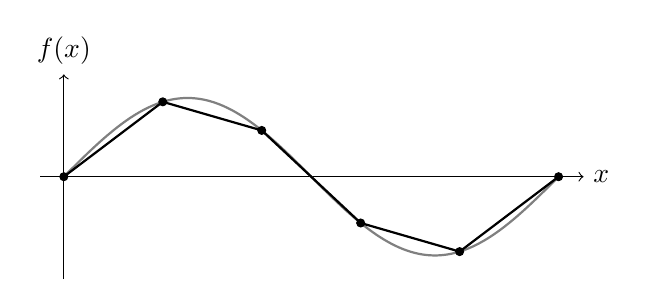
\begin{tikzpicture}
				
				% Axes
				\draw[->] (-0.3,0) -- (6.6,0) node[right] {$x$};
				\draw[->] (0,-1.3) -- (0,1.3) node[above] {$f(x)$};
				
				% Smooth curve f(x) = sin(x), radians
				\draw[gray, thick, domain=0:6.283, samples=100, smooth]
				plot (\x, {sin(\x r)});
				
				% Partition points, evenly spaced, 6 points on [0, 2*pi]
				% x_j = j * 2*pi/5 for j = 0,...,5
				\foreach \j in {0,1,2,3,4,5} {
					\pgfmathsetmacro{\xj}{\j * 2*3.14159/5}
					\pgfmathsetmacro{\yj}{sin(\xj*180/3.14159)} % convert to degrees for TikZ's sin
					\filldraw (\xj,\yj) circle (0.05);
				}
				
				% Interpolant: straight lines connecting consecutive partition points
				\draw[thick]
				plot[mark=none] coordinates {
					(0,{sin(0)})
					(1.2566,{sin(1.2566 r)})
					(2.5133,{sin(2.5133 r)})
					(3.7699,{sin(3.7699 r)})
					(5.0265,{sin(5.0265 r)})
					(6.2832,{sin(6.2832 r)})
				};
				
			\end{tikzpicture}
			\caption{$f(x)=\sin(x)$ on $[0,2\pi]$ (grey) and its piecewise-linear interpolant $I(x)$ (black) through $6$ evenly spaced points (Definition~\ref{def:piecewise-linear-interpolant}). The visible gap between the two curves is exactly what Proposition~\ref{prop:interpolation-error-bound} bounds.}
			\label{fig:uat}
		\end{figure}
		
		\begin{remark}[Representability]
			\label{rem:uat-representability-only}
			Theorem~\ref{thm:uat-1d} shows that a network with the right weights exists, however it says nothing about whether gradient descent (Theorem~\ref{thm:gd-convergence}) can find those weights from a random initialisation, nor how many training steps that would take. \\
			
			The construction here is entirely explicit and non-adaptive, chosen directly from $f$ and a fine enough partition; nothing in this proof involves training a network on data. Universal approximation is a statement about what functions are representable within the network's architecture, not a guarantee about learnability.
		\end{remark}